

\section{Quantitative mass spectrometry: counting molecules}\label{sec:quantification}

This Section lays out procedures for using electrochemistry as a platform for quantification in mass spectrometry. This means relating the signal at a mass-to-charge ratio (m/z) or set of m/z's to the amount of the molecule being quantified, the \textit{analyte}. However, \textit{amount} here can have at least two different meanings.

Mass spectrometry is routinely used to analyze the concentration of analytes in a gas or other matrix\cite{Harris2010, Gross2007}. When the desired value is a concentration in a gas, calibrating the mass spectrometer is trivial. One need only flow a standard gas or series of standard gases with a known concentrations of the analyte past the inlet and measure the signal at a m/z value unique to the analyte. The standard gases should otherwise resemble the gas which will be tested as much as possible. In general, the signal will scale linearly with the concentration, giving a sensitivity factor. Such a sensitivity factor has the dimensions of signal per concentration.

In the context of chip EC-MS and certain other applications such as catalyst testing in microreactors, we mean something different. We use the following definition of quantification:

\begin{definition}
	Quantification: Determining, from mass spectrometer signals, the rate (in molecules per second) at which an analyte is entering the vacuum chamber. \label{d:quantification}
\end{definition} 

Equivalently, quantification means being able to determine the number of molecules that entered the vacuum chamber in a given time from the integrated mass spectrometer signal. In chip EC-MS as well as microreactor experiments, this is useful because all of the products of a catalytic reaction can be assumed to enter the vacuum chamber, and we typically wish to determine the number of catalytic turn-overs from the integrated signal or, at steady state, the turn-over rate from the signal. 

The sensitivity factor we are looking for has the dimensions of integrated signal per molecule. If signal is measured in Amperes and molecules are counted in mol, then the sensitivity factor has units C/mol. Mathematically, the sensitivity factor for analyte $i$ at a mass-to-charge ratio (m/z=) $M$ where there are no interferences, is defined as $F^i_M$ such that:
\begin{align}
S_M &= F_M^i \dot{n}^i_{\text{vac}}\,\hspace{1cm}\text{or, by extension,} \label{eq:S}\\
\int_{t_1}^{t_2} S_M \mathrm{d}t &= F_M^i \Delta n_{\text{vac}} \label{eq:int_S}
\end{align}
where $S_M$ is the signal at m/z=$M$, $\dot{n}^i_\text{vac}$ is the molar flux of analyte $i$ into the vacuum chamber, and $\Delta n_\text{vac}^i$ is the amount of analyte $i$ to enter the vacuum chamber between times $t_1$ and $t_2$.

This type of sensitivity factor is more difficult to determine than the signal-to-concentration sensitivity factor because, given a gas with a known analyte concentration, its determination also requires knowledge of the permeability of the vacuum inlet. Estimating the capillary flux is precisely how quantification was originally accomplished for the microreactors \cite{Henriksen2009} and the electrochemical microreactor which was the predecessor to the EC-MS membrane chip\cite{Trimarco2015}. 

Electrochemistry gives a powerful platform for accurate quantification, because there are analytes for which the electrode current can directly tell us $\dot{n}$. The next Subsection will describe electrochemical calibration, and the following Subsections will describe how electrochemical calibrations can be used to validate calibrations based on capillary flux and together extended to allow quantification, as understood in Definition \ref{d:quantification}, of any analyte.


\subsection{Internal calibration by electrochemistry}\label{subsec:internal}

Electrochemical calibration of mass spectrometer signals is based on establishing a steady and known value for $\dot{n}^i$ in Equation \ref{eq:S} based on Faraday's law of electrolysis:
\begin{equation}
\dot{n}^i_\text{el} = \frac{I}{z\mathcal{F}}\,,\label{eq:Far}
\end{equation}
where $I$ is the current, $z$ is the stoichiometric coefficient of electrons (positive for oxidation and negative for reduction) in the electrochemical half-reaction of which $i$ is a product, and $\mathcal{F}=96487$ C/mol is Faraday's constant.

Equation \ref{eq:Far} implicitly assumes that \textit{all} of the current $I$ goes to formation of the product $i$, i.e. it assumes 100\% \textit{Faradaic efficiency}. Its use is thus limited to reactions that can be run at 100\% Faradaic efficiency. In practice, this is a severe limitation on the analytes that can be calibrated directly by electrochemistry. Three of the analytes that can be calibrated directly are \ch{O2}, \ch{H2}, and \ch{CO2}, which can be produced at $\approx$100\% Faradaic efficiency by OER, HER, and CO oxidation, respectively:
\begin{align}
\ch{2 H2O &-> O2 + 4 (H+ + e- )} &&\text{OER}\label{rxn:OER2}\\
\ch{2 (H+ + e- ) &-> H2} &&\text{HER}\label{rxn:HER2}\\
\ch{CO + H2O &-> CO2 + 2 (H+ + e- )} &&\label{rxn:COox2}\text{CO oxidation}
\end{align}
\begin{figure}[h!]
	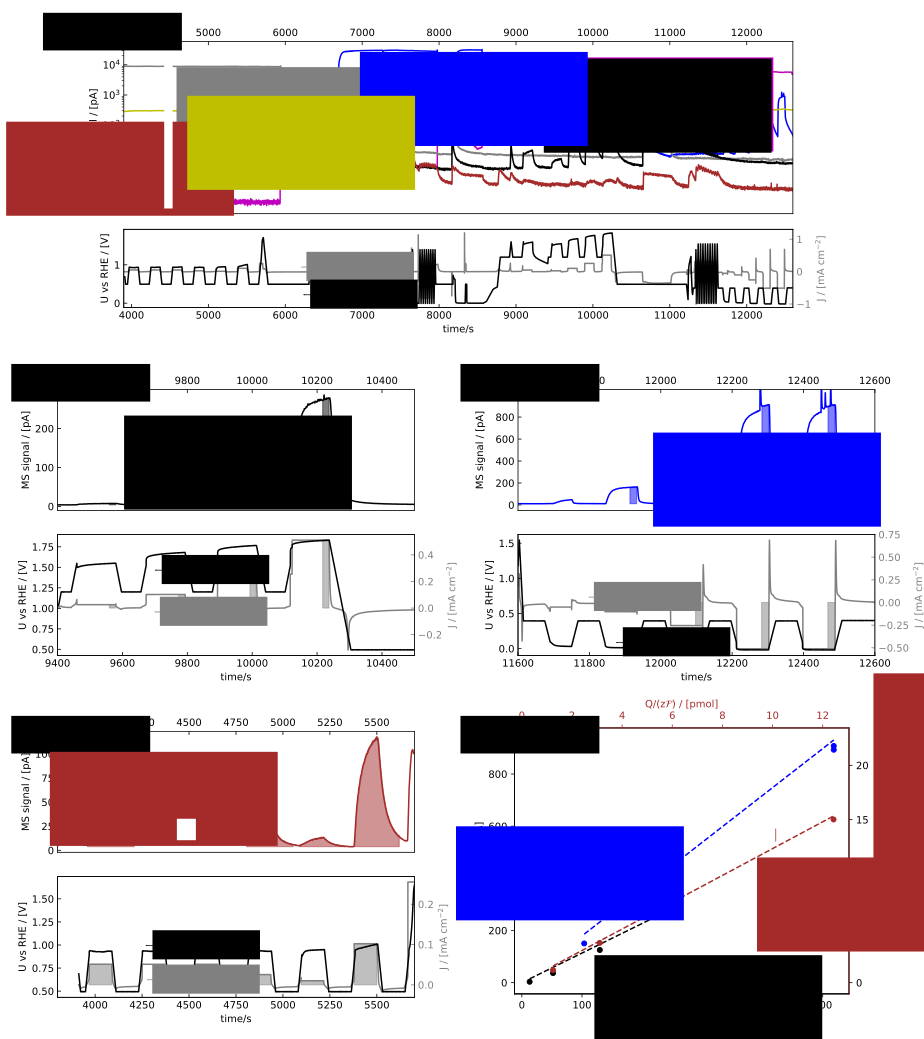
\includegraphics[width=1\textwidth]{02_Tools/fig/internal_calibrations.png}
	\caption{Calibration experiments for \ch{O2} by OER, \ch{H2} by HER, and \ch{CO2} by CO oxidation using a platinum electrode in 1.0 M \ch{HClO4}. \textbf{(a)} The entire experimental dataset. Zoom-ins are shown for the three calibrations: \textbf{(b)}, OER; \textbf{(c)}, HER; and \textbf{(d)} CO oxidation. \textbf{(e)}, The resulting calibration curves are plotted for \ch{H2} and \ch{O2} as near-steady-state signal vs production rate (bottom and left axes), and for \ch{CO2} as integrated signal vs amount produced (top and right axes). The proportionality between the two x-axes and the two y-axes are identical such that the slopes, which are the respective sensitivity factors, are directly comparable.
	}
	\label{fig:internals}
\end{figure}
Figure \ref{fig:internals} shows calibrations for \ch{O2}, \ch{H2}, and \ch{CO2} by these reactions. These calibration data are not as flawless as those in the SI to Paper \ref{Trimarco2018}. They were chosen for this Thesis because, together with the data in Figure \ref{fig:internals_2} below, which were taken on the same day, they include the largest number of directly comparable calibrations. I collected the data in Figures \ref{fig:internals} and \ref{fig:internals_2} together with Anna Winiwarter to obtain a full set of sensitivity factors to calibrate the results of propene stripping experiments that build on the results in Paper \ref{Winiwarter2019}.

The full dataset is shown in Figure \ref{fig:internals}a. From the left: the dataset starts with the electrode in \ch{CO}-saturated electrolyte. The electrode is subject to several periods of 2 minutes of constant-current CO oxidation, inter-spaced by scans to a \textit{resting potential} of 0.5 V vs RHE to separate the peaks. There is a small gap in the MS data around 4500s due to a computer glitch. After the \ch{CO2} calibration, the carrier gas is changed from \ch{CO} to He, and then to \ch{H2} to measure the signal due to \ch{H2} carrier gas flux through the capillary (which will be discussed in Subsection \ref{subsec:capillary}) and to calibrate the reference electrode. (We actually realize after the anodic scan at $\approx$ 7700 s that we had forgotten to strip off the adsorbed \ch{CO} from before, which would have poisoned the electrode for HER/HOR, and so we repeated the RHE calibration.) Then the carrier gas was changed back to \ch{He} for \ch{O2} calibration by OER. Again, we used 2-minute constant current steps inter-spaced by time at a resting potential to get separated peaks in the m/z=32 signal. Then we switched the carrier gas briefly to \ch{O2} to measure the signal due to \ch{O2} carrier gas flux through the capillary, and switched back to \ch{He}. Finally, after cycling the potential to clean off any contaminants that may have adsorbed or deposited on the electrode, we calibrated \ch{H2} by HER, again with constant-current measurements inter-spaced by a resting potential.

There are two ways of extracting a sensitivity factor from calibration data made with constant-current calibration steps inter-spaced by resting periods: differential and integral. For a differential calibration, we chose a time interval over which to make the assumption of steady-state, i.e. 
\begin{equation}
\dot{n}^i_\text{vac} = \dot{n}^i_\text{el}\,,\label{eq:SS}
\end{equation}
and the sensitivity factor $F_M^i$ is, according to Equation \ref{eq:S}, simply the ratio of the signal $S_M$ to the production rate $n^i_\text{el}$, where the latter is calculated by Equation \ref{eq:Far}. For an integral approach, we do not make the assumption of steady state, but instead use the fact that, over time, every gas molecule formed at the electrode will make it to the vacuum chamber:
\begin{equation}
\int \dot{n}^i_\text{vac}\mathrm{d}t = \int \dot{n}^i_\text{el}\mathrm{d}t\,,\label{eq:int}\,
\end{equation}
and then determine $F_M^i$ by Equation \ref{eq:int_S}.

The differential approach is usually good enough for \ch{O2} (Figure \ref{fig:internals}b) and \ch{H2} (Figure \ref{fig:internals}c), which have fast mass transport [Paper \ref{Trimarco2018}] and can reach steady state within a minute. In this particular dataset, the mass transport is rather slow, perhaps due to poor alignment of the electrode, and the respective signals appear to be close to but not quite at steady state. It turns out that it's good enough (using the integral approach results in the same sensitivity factor within 2\%). The highlighted areas of Figure \ref{fig:internals}b and c show the time interval over which the signal was averaged.

For \ch{CO2} (Figure \ref{fig:internals}d), which has much slower mass transport due to its higher solubility in the electrolyte [Paper \ref{Trimarco2018}], we have to use the integral approach. Here, the highlighted areas show the time intervals for which $\dot{n}^{\ch{CO2}}_\text{el}$ (bottom panel) and $S_\text{M44}$ (top panel) were taken. The two calibration points affected by the gap in the MS data were excluded.

The resulting calibration curves are plotted in Figure \ref{fig:internals}e. The top x-axis and right y-axis are in integrated units, for \ch{CO2}. The proportionality between the two x-axes and the two y-axes are identical such that the slopes, which are the respective sensitivity factors, are directly comparable. The sensitivity factors, resulting from least-squares-fitting without forcing through zero, are shown. The lines shown have the sensitivity factor as their slope but \textit{are} forced through zero, to show a typical non-ideality typical of these calibration curves: there is a small, approximately constant, offset. This offset implies that there is some charge passed through the electrode which cannot be accounted for by Reactions \ref{rxn:OER2}, \ref{rxn:HER2}, and \ref{rxn:COox2}. In all cases, it can possibly be attributed to processes oxidizing or reducing the electrode, or adsorbing or desorbing species from its surface. This illustrates the importance of always being critical of the assumptions of 100\% Faradaic efficiency, even for simple reactions, and using multiple current densities for calibration.
\begin{figure}[h!]
	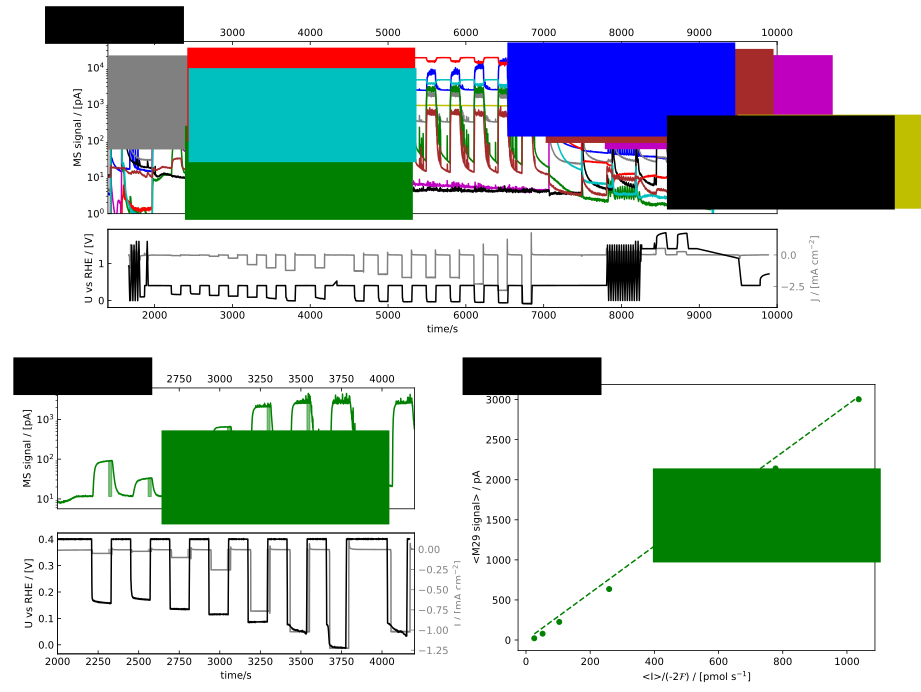
\includegraphics[width=1\textwidth]{02_Tools/fig/internal_calibrations_2.png}
	\caption{Calibration experiment for propane (\ch{C3H8}) by reduction (hydrogenation) of propene (\ch{C3H6}) on Pt in 1.0 M \ch{HClO4}. \textbf{(a)} The entire experimental dataset, taken immediately after that in Figure \ref{fig:internals}a. \textbf{(b)}, A zoom-in is shown for the propane calibration. The data points at larger current, where propene reduction is mass-transport limited and some of the current goes to HER are excluded. \textbf{(c)}, The resulting calibration curve is plotted as near-steady-state signal vs production rate.
	}
	\label{fig:internals_2}
\end{figure}
Once a sensitivity factor $F_M^i$ is determined, it can be used to calculate the flux of $i$ from the signal at $M$ according to:
\begin{equation}
\dot{n}^i_{\text{vac}} = \frac{1}{F_M^i} S_M = C_M^i S_M\,,
\end{equation}
where $C_M^i$ is a \textit{calibration factor}, which in this simple case is just the reciprocal of the sensitivity factor.

Figure \ref{fig:internals_2} shows a calibration for an additional reaction that can be run at 100\% Faradaic efficiency on platinum: the propene reduction reaction, Reaction \ref{rxn:PRR}:
\begin{equation}
\ch{C3H6 + 2 (H+ + e- ) -> C3H8}\label{rxn:PRR}
\end{equation}
I first encountered this reaction while doing the propene striping experiments reported in Paper \ref{Winiwarter2019}. Briefly, we found that the tendency of adsorbed propene to strip off from a palladium surface as propane or propene on a cathodic sweep correlates with the coverage on the surface, motivating a mechanism for the propene oxidation reaction (the main subject of that paper) in which surface coverage guides the reaction pathway towards certain intermediates.  This is, in my opinion, a fantastic story, and was a great project to be part of, though it is out of the scope of this Thesis. I highly recommend the paper to an interested reader of this Thesis. Anna Winiwarter has since expanded on those EC-MS experiments to probe propene reactivity. However, propene reduction is included here only because it demonstrates well some of the challenges and opportunities in quantitative EC-MS.

The first challenge in quantification of propane and propene is that there is a significant overlap in their mass spectra (Figure \ref{fig:spectra}). Propane can itself be detected and quantified without interference at its most prominent mass fragment, m/z=29. The sensitivity factor of propane at m/z=29, $F_{\text{M29}}^{\ch{C3H8}}$, is determined by Faradaic propene reduction in Figure \ref{fig:internals_2}b and c. 
\begin{figure}[h!]
	\centering
	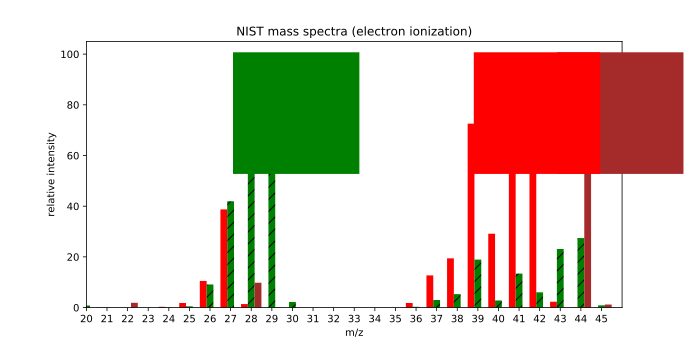
\includegraphics[width=0.75\textwidth]{02_Tools/fig/mass_spectra.png}
	\caption{Mass spectra of propene (\ch{C3H6}, red), propane (\ch{C3H8}, green and hatched), and \ch{CO2} (brown) from NIST\cite{NIST}
	}
	\label{fig:spectra}
\end{figure}
However, propane interferes with two other molecules of interest at their most prominent mass fragments: propene at m/z=41 and \ch{CO2} at m/z=44.

To deal with this, using \ch{CO2} as an example: In situations where both propane and \ch{CO2} are present, we should subtract the portion of the m/z=44 signal which is due to propane before dividing by $F_\text{M44}^{\ch{CO2}}$ to get the \ch{CO2} flux. The m/z=44 signal which is due to propane can, in turn, be calculated from the m/z=29 signal, which is solely due to propane. Mathematically,
\begin{align}
\dot{n}^{\ch{CO2}}_{\text{vac}} &= \frac{1}{F^{\ch{CO2}}_\text{M44}}S^{\ch{CO2}}_\text{M44}\\
&= \frac{1}{F^{\ch{CO2}}_\text{M44}}\left(
S_\text{M44} - S^{\ch{C3H8}}_\text{M44}
\right)\\
&= \frac{1}{F^{\ch{CO2}}_\text{M44}}\left(
S_\text{M44} - \frac{I^{\ch{C3H8}}_\text{M44}}{I^{\ch{C3H8}}_\text{M29}}S^{\ch{C3H8}}_\text{M29}
\right)\\
&= \frac{1}{F^{\ch{CO2}}_\text{M44}}S_\text{M44} - \frac{I^{\ch{C3H8}}_\text{M44}}{F^{\ch{CO2}}_\text{M44}I^{\ch{C3H8}}_\text{M29}}S_\text{M29}\,,
\end{align}
where $I_M^i$ is the relative intensity at m/z=$M$ for in the mass spectrom of analyte $i$. These are taken from NIST. 

The substitution of $S_\text{M29}$ for $S^{\ch{C3H8}}_\text{M29}$ assumes that all of the signal at m/z=29 is due to propane.

Another way to write this is 
\begin{align}
\dot{n}^{\ch{CO2}}_{\text{vac}} = C_\text{M44}^{\ch{CO2}} S_\text{M44} + C_\text{M29}^{\ch{CO2}} S_\text{M29}
\,\hspace{5mm}\text{with}\\
C_\text{M44}^{\ch{CO2}} = \frac{1}{F_\text{M44}^{\ch{CO2}}}\hspace{5mm}\text{and}\hspace{5mm} C_\text{M29}^{\ch{CO2}} = - \frac{I^{\ch{C3H8}}_\text{M44}}{F^{\ch{CO2}}_\text{M44}I^{\ch{C3H8}}_\text{M29}}
\end{align} 
In general, we can write 
\begin{align}
\dot{n}^{i}_{\text{vac}} = \sum_M C_M^i S_M\,,
\end{align}
or, in vector form:
\begin{align}
\dot{n}^{i}_{\text{vac}} = \mathbf{C}^i \cdot \mathbf{S}
\end{align}

The \texttt{Molecule} class of the \texttt{EC\_MS} python package (Appendix \ref{app:EC_MS}) implements both the simple ($F_M^i$) and vectorized ($\mathbf{C}^i$) quantification techniques presented above. Fortunately, it is for only a few projects that I've had to use the vectorized approach, and this does not include any of the isotope-labeling studies presented later in this Thesis.


\subsection{External calibration based on the capillary flux}\label{subsec:capillary}

The determination of the sensitivity factors $F_M^i$ by Faradaic production of analyte $i$ described in the previous Subsection is referred to as \textit{internal calibration}, since all of the molecules giving the signal in the calibration experiment are made inside the working volume of the EC-MS setup, and the amount of analyte is known. Here, we describe \textit{external calibration}, whereby a carrier gas, originating outside the setup (in a bottle, or, in the case of air, from the room), is leaked through the capillary of the chip and into the mass spectrometer. The challenge then, to determine a sensitivity factor $F_M^i$ enabling quantification by Definition \ref{d:quantification}, is to determine the flux through the capillary of analyte $i$ given the composition of the gas in the chip. In other words, it is to determine the \textit{capillary flux}. 

The flow of molecules through the capillary goes through at least three regimes as the pressure droops from 1 bar to high vacuum\cite{Henriksen2009}: (1) a viscous flow regime near ambient pressure, (2) a transition regime, and (3) a molecular flow regime governed by Kundsen diffusion near high vacuum. It is therefor not trivial to derive an analytical expression, but this has been done. It is\cite{Trimarco2017_PhD}:
\begin{equation}
\dot{n}_{\mathrm{cap}} = \frac{1}{R T}\frac{1}{l_\text{cap}} 
\left(\left( 
\frac{\pi}{8\nu}a^4\bar{p} + \frac{2\pi}{3}a^3\bar{v} \frac {1+2\frac{2\sqrt{2}}{\sqrt{\pi}}\frac{a}{\eta}\frac{\bar{p}}{\bar{v}}} {1+2.48\frac{2\sqrt{2}}{\sqrt{\pi}}\frac{a}{\eta}\frac{\bar{p}}{\bar{v}}}
\right)
\left(p_1-p_{\mathrm{tran}}\right) 
+ 
\frac{2\pi}{3}a^3\bar{v}\left(p_{\mathrm{tran}}-p_2\right)\right) 
\;, \label{eq:capillary}
\end{equation}
Here, $p_1$ is the inlet pressure (usually 1 bar), $p_2$ is the outlet pressure ($\approx$ 0), $p_{\mathrm{tran}}=\frac{k_B T}{2 \sqrt{2}\pi s^2 a}$ is the pressure at which the transition from viscous to molecular flow occurs, $\bar{p}=\frac{p_1 + \bar{p}_{\mathrm{tran}}}{2}$ is the average pressure in the viscous flow regime, $\eta$ is the viscosity of the gas, $s$ is the molecular diameter, $\bar{v}=\sqrt{\frac{8 k_B T}{\pi m}}$ is the mean thermal velocity of the gas molecules, and $m$ is the molecular mass. Furthermore, $l_\text{cap}$ is the length of the capillary, and $a=h_\text{cap}=w_\text{cap}$ is its height and width, assumed to be equal (square cross-section). By design, $l_\text{cap} = 1\,\text{mm}$, $l_\text{cap} = 6\,\mu\text{m}$, and $h_\text{cap} = 6\,\mu\text{m}$.

This equation has been validated experimentally for a microreactor by sealing the outlets of an interface block and measuring the rate at which the pressure dropped as air leaked through the chip's capillary into the vacuum chamber\cite{Henriksen2009}.

With the internal calibration described in the previous Subsection, however, there is an easier and more precise way to validate the capillary flux: compare the signal due to a molecule in the carrier gas to the signal when the same molecule is produced electrochemically. This is most easily, and most often, done for \ch{O2}, as \ch{O2} can be produced electrochemically with near-100\% Faradaic efficiency, and is also present in air, giving a ``free'' carrier gas measurement.

In the dataset presented in the previous Subsection, an air measurement is provided at the very beginning (i.e. t$\approx$ 1500 s) of Figure \ref{fig:internals_2}. Here, the m/z=32 signal is 1.88$\cdot 10^{-9}$ A. The \ch{O2} flux, based on the sensitivity factor $F$ calibrated internally, is
\begin{equation}
\dot{n}^{\ch{O2}}_\text{cap} = \frac{S_\text{M32}}{F^{\ch{O2}}_\text{M32}} = \frac{1.88\cdot 10^{-9} \text{[A]}}{1.11 \left[\frac{\text{C}}{\text{mol}}\right]} = 1.70 \left[\frac{\text{nmol}}{\text{s}}\right]
\end{equation}
Using the value of $x^{\ch{O2}}_\text{air}=20.95$\% for the \ch{O2} content of air and assuming that there is not significant separation effect on the gases in air by the capillary, the capillary flux of air is 
\begin{equation}
\dot{n}^{\text{air}}_\text{cap} = \frac{\dot{n}^{\ch{O2}}_\text{cap}}{x^{\ch{O2}}_\text{air}} = 8.08 \left[\frac{\text{nmol}}{\text{s}}\right]\,.
\end{equation}
In contrast, the flux of air through the capillary predicted by Equation \ref{eq:capillary}, using the design parameters for $l_\text{cap}$, $h_\text{cap}$, and $w_\text{cap}$, is 6.86 nmol/s. How do reconcile this difference? In reality, it is $h_\text{cap}$ which varies from capillary to capillary. This is a result of non-uniformity in the deep-reactive-ion-etching step that forms the capillary\cite{Trimarco2017_PhD}. The actual capillary height, as measured by profilometry in the clean room, can vary by $\approx$ 20 \% across a wafer, which leads to varying permeability, and thus varying air flux. 

In fact, calibrating the \ch{O2} signal at m/z=32, and then measuring the m/z=32 signal in air is a way to \textit{calibrate the chip capillary}. Since the real variation in the capillary flux is due to variation in the capillary height, the most correct way to account for it would be to solve Equation \ref{eq:capillary} for $h_\text{cap}$ with the measured $\dot{n}_\text{cap}^\text{air}$. However, in practice (so far), to make the implementation easier, we incorporate the difference in an effective capillary length:
\begin{equation}
l_\text{eff} = \frac{\dot{n}^{\text{air}}_\text{cap, pred.}}{\dot{n}^{\text{air}}_\text{cap, meas.}} l_\text{cap}= \frac{6.86 \left[\frac{\text{nmol}}{\text{s}}\right]}{8.08 \left[\frac{\text{nmol}}{\text{s}}\right]} 1.00\,\text{[mm]} = 0.85\,\text{[mm]}
\end{equation}
If $l_\text{eff}$ is used instead of $\l_\text{cap}$ for in Equation \ref{eq:capillary}, the equation predicts the ``correct'' value for the flux of air, i.e. the measured flux as calibrated by OER. 

With the chip thus calibrated, we can use Equation \ref{eq:capillary} with $l_\text{eff}$ to calculate the capillary flux of any gas $i$, given its dynamic viscosity $\eta^i$, molecular diameter $s^i$, and molecular mass $m^i$. All that is then needed is a mass spectrometer signal at an m/z=$M$ without interference using $i$ as a carrier gas, and we can calculate its sensitivity factor $F_M^i$. The datasets presented in Figures \ref{fig:internals}a and \ref{fig:internals_2}a include the necessary data for such external calibration of several gases. The results are shown in Table \ref{tab:externals}. When possible, the sensitivity factor determined by electrochemistry is included for comparison. While the internal and external calibrations for \ch{O2} in air match by the definition of $l_\text{eff}$, the agreement for \ch{H2} and \ch{CO2} is also quite good, validating the method.

\begin{table}
	\centering
	\begin{tabular}{c|c|c|c|c|c||c|c|c|c||c}
		Molecule & $\eta$ & $s$ & $m$ & $x^i$ & $\dot{n}_\text{cap}^i$ & dataset & time & m/z=$M$ & $F_M^i$ & $F_M^i$ (EC) \\
		& / [$\mu$Pa$\cdot$s] & / [\AA] & / [amu]& & / [nmol/s] & & / [s]& & / [C/mol] & / [C/mol] \Bstrut\\
		\hline
		\ch{O2} in air & 18.5 & 3.66 & 30.0 & 0.2095 & 1.70 & 
		 \ref{fig:internals_2}a & 1525 & 32 & 1.11 & 1.11 \Tstrut\\
		\ch{N2} in air & 18.5 & 3.66 & 30.0 & 0.7808 & 6.33 & 
		 \ref{fig:internals_2}a & 1525 & 28 & 1.42 & - \\
		\ch{Ar} in air & 18.5 & 3.66 & 30.0 & 0.0093 & 0.0755 & 
		 \ref{fig:internals_2}a & 1525 & 40 & 0.98 & - \\
		\ch{He} & 20.0 & 2.15 & 4.0 & 1 & 8.64 & 
		 \ref{fig:internals}a & 10400 & 4 & 0.71 & - \\
		\ch{CO} & 17.8 & 3.76 & 28.0 & 1 & 7.14 & 
		 \ref{fig:internals}a & 5000 & 28 & 1.24 & - \\
		\ch{H2} & 8.9 & 2.71 & 2.0 & 1 & 16.50 & 
		 \ref{fig:internals}a & 7200 & 2 & 1.83 & 1.81 \\
		\ch{O2} & 20.7 & 3.55 & 32.0 & 1 & 6.24 & 
		 \ref{fig:internals}a & 10900 & 32 & 1.04 & 1.11 \\
		\ch{CO2} & 15.0 & 4.53 & 44.0 & 1 & 9.38 & 
		 \ref{fig:internals_2}a & 9850 & 44 & 1.32 & 1.23 \\
		\ch{C3H6} & 8.85 & 4.50 & 42.1 & 1& 15.11 & 
		 \ref{fig:internals_2}a & 4400 & 41 & 1.22 & - \\
	\end{tabular}
\caption{External calibrations. The flow properties of the carrier gas $\eta$, $s$, and $m$ as well as the fraction $x^i$ of component $i$ are used to calculate the flux of $i$ through the capillary, $\dot{n}^i_\text{cap}$. This is compared to the measured signal at a given m/z in a given dataset, where the dataset refers to Figure \ref{fig:internals} or \ref{fig:internals_2} of the previous Subsection. Dataset \ref{fig:internals} was taken with a chip with $l_\text{eff}=0.99$ mm and Dataset \ref{fig:internals_2} was taken with a chip wtih $l_\text{eff}=0.86$ mm, $l_\text{eff}$ being used to calculate $\dot{n}^i_\text{cap}$. The signal at m/z=$M$ was averaged over 50 s centered at the time indicated, chosen for a steady interference-free measurement. The sensitivity factor $F_M^i$ is the ratio of that signal to $\dot{n}_\text{cap}^i$. This is compared, when possible, to $F_M^i$ calculated by electrochemical (internal) calibration.
}
\label{tab:externals}
\end{table}



\subsection{Sensitivity factors from theory, and non-ideal effects}\label{subsec:MS_theory}

The \textit{internal} and \textit{external} calibration methods described above, linked via $l_\text{eff}$, enable the determination of sensitivity factors for any analyte which can either be produced electrochemically with 100\% Faradaic efficiency or flowed through the chip as a carrier gas. However, these conditions often exclude analytes of interest. If sensitivity factors could be \textit{predicted} through first principles, then any analyte could be quantified. In this Subsection, I propose such a method and check its ability to predict the variation in the sensitivity factors determined in the previous two Subsections.

It is hard to find anything in the literature about predicting mass spectrometry sensitivity from first principles, not least because applications requiring quantification as understood by Definition \ref{d:quantification} are quite rare. The following steps happen between a molecule $i$ entering the vacuum chamber and a signal at m/z=$M$ being registered (Figure \ref{fig:MS})\cite{Gross2007}:
\begin{itemize}
	\item
	The molecule must reach the filament
	\item
	The molecule must be ionized by the filament
	\item
	The ionization must result in a fragment at m/z=$M$
	\item
	The fragment must be transmitted through the quadrupole while it is filtering for m/z=$M$
	\item
	The fragment starts an electron cascade on the channel electron multiplier
\end{itemize}
The signal $S_M$ (in A) can thus in principle be related to the flux $\dot{n}^i_\text{vac}$ by a series of probibilites $P$ and the CEN amplification $A$:
\begin{equation}
S_M = \dot{n}^i_\text{vac} P_\text{filament} P_\text{ionize}(i) P_\text{fragment}(i, M) P_\text{transmission}(M) A(M)\,,
\end{equation}
Where I've tried to indicate whether each probability depends on the identity of the molecule $i$ or the mass of the fragment $M$.

The probability of reaching the filament $P_\text{filament}$ depends a lot on the geometry of the vacuum chamber, notably where the inlet, filament, and pump are in relation to each other. I'll assume that it doesn't depend on $i$ or $M$. The ionization probability $P_\text{ionization}(i)$ is proportional to the ionization cross section $\sigma^i$ of analyte $i$, which is generally available in the literature. It depends on the ionization energy, which is 70 eV for all of the work in this PhD thesis. The probability of a given fragment being formed after the molecule is ionized can be calculated from the mass spectrum:
\begin{equation}
P_\text{fragment}(i, M) = \frac{I_M^i}{\sum_{M'}I_{M'}^i}
\end{equation}
where $I_{M'}^i$ is the intensity of mass fragment $M'$ in the electron ionization mass spectrum of analyte $i$. These mass spectra, which also depend on the ionization energy, are often available at NIST\cite{NIST}. They can also be measured directly in the EC-MS setup if $i$ is available as a carrier gas. 

The processes after fragmentation can be assumed to only depend on the fragment mass-to-charge ratio $M$. Both of these processes, quadrupole transmission and CEM amplication factor, will also depend on the ion acceleration, which is {\color{red}???} throughout this PhD project. They can be grouped into a function $T(M)$ which I will refer to as the \textit{transmission function}, implying that the transmission through the quadrupole is gives most of the mass dependence, even though I'm not sure this is true.

\begin{figure}[h!]
	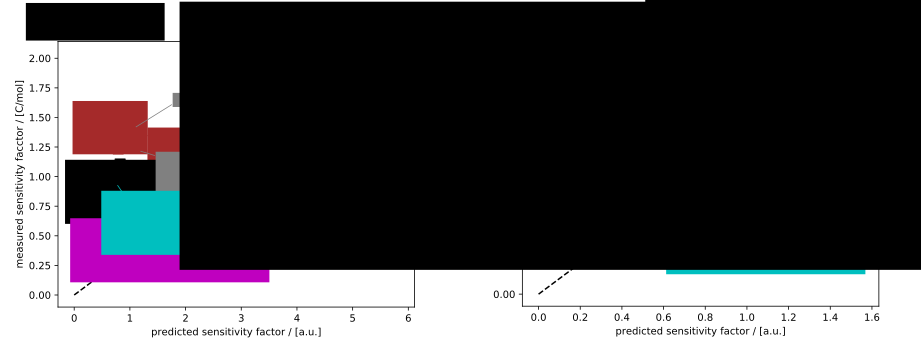
\includegraphics[width=\textwidth]{02_Tools/fig/calibration_results.png}
	\caption{Measure sensitivity factor $F_M^i$ vs predicted sensitivity factor $f_M^i$ for two guesses at the transmission function: \textbf{(a)}, inversely proportional with the m/z ratio; and \textbf{(b)}, inversely proportional with the square root of the m/z ratio. The measured sensitivity factors, which are shown in Table \ref{tab:externals}, are determined via capillary flux (triangles) or an electrochemical reaction (squares). }
	\label{fig:transmission}
\end{figure}

Overall, then, the predicted sensitivity factor, which is denoted with a little $f$ to distinguish it from the experimentally determined big $F$, is
\begin{equation}
f_M^i = \frac{S_M}{\dot{n}^i_\text{vac}} = k \sigma_i \frac{I_M^i}{\sum_{M'}I_{M'}^i} T(M)\,.\label{eq:rsf}
\end{equation} 
Where $k$ is a proportionality factor, which I choose to set $f_{\text{M28}}^{\ch{N2}} = 1$. The challenge, then, is to determine $T(M)$.

Some hints can be found from quadrupole theory\cite{Douglas2009}: For a quadrupole mass analyzer, the transmission function should correlate inversely with the resolution $R = M / \Delta M$. A perfectly-tuned mass spectrometer should have a constant mass resolution resolution, i.e. $\Delta M = c$. If so, the resolution varies directly with $M$. This implies that the transmission function should vary inversely with $M$, i.e., $T(M)=M^{-1}$.

Figure \ref{fig:transmission}a shows the measured $F_M^i$ plotted against the thus-calculated $f_M^i$ with $T(M)=M^{-1}$. The predictive scheme does a terrible job at explaining the variation in the data.

If we keep the form of the transmission function and change the exponent, we can get a relatively good fit by putting the exponent to -1/2. This may indicate that the CEM amplication factor scales with $M^{+1/2}$, or may indicate that the above reasoning doesn't quite hold. In any case, $T(M)=M^{-1/2}$ seems to give a good fit. The best-fit line of proportionality between $F$ and $f$ gives a root-mean-square error on the prediction of $F$ of 12\%. In other words, we can quantify an arbitrary new analyte $i$ at mass $M$ to within about 12\% accuracy (20\% to be generous) without a new calibration. We have developed a generalized solution to the problem of quantification as understood by Definition \ref{d:quantification}!
\vspace{5mm}

There is, however, an important exception: if the carrier gas influences the sensitivity of the mass spectrometer, then all bets are off. This actually seems to be the case when propene is the carrier gas. Figure \ref{fig:internals_2} shows an internal calibration for propane by propene reduction. In the higher-current steps in Figure \ref{fig:internals_2}a, propene reduction is mass-transport limited and hydrogen is also produced. Assuming that there are no Faradaic processes other than propene reduction to propane and hydrogen evolution, the amount of hydrogen produced can be determined from the electrode current and the calibrated propane signal. Figure \ref{fig:propene_transmission}a shows the data used to test the \ch{H2} calibration in propene, calibrated using the \ch{H2} sensitivity factor calculated in He. Faradaic analysis shows that the \ch{H2} signal is consistently $\approx 3$ times larger than expected based on subtracting the calibrated propane signal from the total current density, and using the calibration of \ch{H2} at m/z=2 by HER in He carrier gas. This implies that the sensitivity factor of \ch{H2} at m/z=32 ($F_\text{M2}^{\ch{H2}}$) with propene as the carrier gas is $\approx 3$ times larger than it is with He as a carrier gas. The sensitivity factors for \ch{H2} at m/z=2 and for propane at m/z=29 are included, versus the sensitivity factors predicted by Equation \ref{eq:rsf} with $T(M)=M^{-1/2}$, in Figure \ref{fig:propene_transmission}b. They are both way above the trendline set by the calibration factors measured in other carrier gases.
\begin{figure}[h!]
	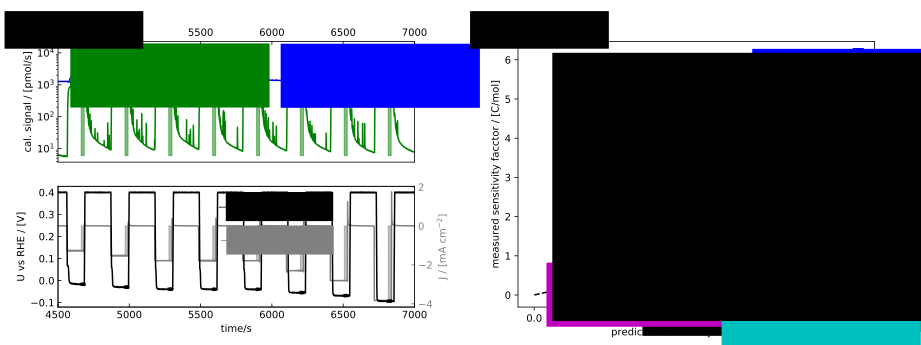
\includegraphics[width=\textwidth]{02_Tools/fig/H2_in_propene_experiment.png}
	\caption{Non-ideality with propene as carrier gas: \textbf{(a)}, Propene reduction + HER, data from Figure \ref{fig:internals_2}a. \textbf{(b)}, Measured vs predicted calibration factors including propane at m/z=29 measured by propene reduction and \ch{H2} at m/z=2 measured by HER in propene, which do not fit the trend of the other masses. A transimission function of $T(M) = M^{-1/2}$ was used for the predicted calibration factor. Propene was measured at m/z=41 and propane at m/z=29. The others analytes are measured at the same masses as in Figure \ref{fig:transmission}. The green dot shows the prediction for the sensitivity factor of propane at m/z=29.}
	\label{fig:propene_transmission}
\end{figure}

These unpredictable and therefore undesireable effects of propene on the mass spectrometer sensitivities are likely due to space-charge effects. Propene has the highest capillary flux of the carrier gases used (Table \ref{tab:externals}) due to its low viscosity, and has a rather high ionization cross-section. This results in a high concentration of ions in the mass spectrometer, which apparently leads to generally increased sensitivity, though I do not claim to understand why. Nonetheless, the response at m/z=29 is linear with propane production rate (Figure \ref{fig:internals_2}c, indicating that quantification of propane using this sensitivity factor is valid when propene is the carrier gas.

The question is then: what to do if we want to quantify propane in another carrier gas? This is, in fact, what we wished to do for the propene stripping experiments in Paper \ref{Winiwarter2019}, where the interesting signal is the propane that comes off in inert gas after propene has been adsorbed on the surface. I think the best strategy is to predict the sensitivity factor for propane in He based on the other calibrations and the trendline in Figure \ref{fig:transmission}b. This prediction is indicated by the green dot in Figure \ref{fig:propene_transmission}b. Whereas propene reduction to propane gives a sensitivity factor of $F^{\ch{C3H8}}_\text{M29} = 2.93$ C/mol, the theory presented in this Subsection indicates the calibration factor in He is $F^{\ch{C3H8}}_\text{M29} = 1.3$ C/mol (to within $\approx$ 20\%). We had not yet understood this effect of propene on the overall sensitivity of the mass spectrometer when publishing Paper \ref{Winiwarter2019}, and thus likely underestimated the amount of propane desorbed in the striping experiments reported there by a factor of $\approx 2$.


\subsection{Quantitative mass spectrometry in practice - methanol synthesis and CO reduction}\label{subsec:in_practice}

The aim of this Subsection is to provide practical suggestions on how to use the calibration methods described in the previous Subsections for users of EC-MS and other techniques benefiting from quantification as understood by Definition \ref{d:quantification}. Let's say you want to quantify a gaseous analyte $i$. First you need to find a mass-to-charge ratio $M$ at which no other molecules in your experiments will give a signal, or at least where you expect the interference to be manageable (as described in the end of Subsection \ref{subsec:internal}). The goal then is to determine the sensitivity factor $F_M^i = S_M/\dot{n}^i_\text{vac}$. You have three options, none of which excludes the others:
\begin{enumerate}
\item \textit{Internal calibration}, Subsection \ref{subsec:internal}: If you can produce a known number of molecules of your analyte by an electrochemical reaction, then do so, and measure the signal! This is the most certain way to get a sensitivity factor, as it relies on no assumptions other than Faraday's law of electrolysis (Equation \ref{eq:Far}) to determine $\dot{n}^i_\text{el}$, which is equal to $\dot{n}^i_\text{vac}$ at steady-state or when integrated. A drawback is if a reactant gas is needed which won't be the carrier gas during the measurements you wish to quantify, since in some cases the carrier gas can influence the sensitivity factors. Furthermore, knowing how many molecules you produced generally requires being able to assume 100\% Faradaic efficiency. In my experience, there is often a small but constant amount of residual current from some other process, so internal calibration should use several different current densities and use the slope of the line-of-best-fit between the measured $S_M$ and expected $\dot{n}^i_\text{el}$ as the sensitivity factor. 

Internal calibration is implemented with the function \texttt{calibration\_curve} of the \texttt{EC\_MS} python package (Appendix \ref{app:EC_MS}). This function also produces plots of the types in Figure \ref{fig:internals}b-e.

\item 
\textit{External calibration}, Subsection \ref{subsec:capillary}: If you have $i$ available as a gas, either pure or diluted, then you can fill the chip with this gas and measure the signal at $M$. However, this requires that you know the capillary flux through the chip. The capillary flux can be calculated by Equation \ref{eq:capillary}, but only if the capillary dimensions are known, and in practice these dimensions vary a bit from chip to chip. Thus, external calibration requires a \textit{chip calibration}, described below. 

External calibration is implemented with the function \texttt{point\_calibration} of the \texttt{EC\_MS} python package (Appendix \ref{app:EC_MS}).
\begin{itemize}
	\item \textit{Chip calibration}, Subsection \ref{subsec:capillary}: A chip calibration means determining the effective capillary length $l_\text{eff}$ that can take the place of $l_\text{cap}$ in Equation \ref{eq:capillary} so that it predicts the measured flux of an analyte with an internal calibration. Typically, this means determining $F_\text{M32}^{\ch{O2}}$ using OER, and then measuring the m/z=32 signal while the chip is open to air.
	
	Chip calibration is implemented with the function \texttt{chip\_calibration} of the \texttt{EC\_MS} python package (Appendix \ref{app:EC_MS})
\end{itemize}
\item 
\textit{Predictive calibration}, Subsection \ref{subsec:MS_theory}. If a number of other sensitivity factors, $F_{N}^{j}$, can be obtained by internal or external calibration, then these other sensitivity factors can be used to predict $F_M^i$. A predicted calibration $f_N^j$ is calculated for each other molecule $j$ according to Equation \ref{eq:rsf}. This requires knowledge of the ionization cross-sections and mass spectra of all the analytes (available in the literature, usually at NIST\cite{NIST}) and a \textit{transmission function} $T(M)=M^x$ describing the dependence of the sensitivity on the mass fragment. $T(M)$ depends on the tuning of the mass spectrum, and at the setup used for this PhD project, $T(M)=M^{-1/2}$ works well. As many internal and external calibrations as possible should be used to fit and build confidence in $T(M)$. Once a line of proportionality $F_N^j = a f_N^j$ is established, $F_M^i$ is predicted by calculating $f_M^i$ by Equation \ref{eq:rsf} and multiplying by $a$. 

Predictive calibration is implemented with the function \texttt{recalibrate} of the \texttt{EC\_MS} python package (Appendix \ref{app:EC_MS}). This function also produces plots of the type in Figure \ref{fig:transmission}. 

\end{enumerate}

Ideally, at the start of a research project, all three of the above strategies should be used for as many analytes of interest as possible. Plotting $F$ against $f$ will help find non-ideal effects such as that described for propene as a carrier gas in Subsection \ref{subsec:MS_theory}.

Notice that predictive calibration relies on calibrating as many molecules as possible by external calibration or internal calibration in order to determine $T(M)$ and the proportionality between $F$ and $f$. Note also that external calibration depends on a chip calibration which in turn depends on an internal calibration. And internal calibration relies on using the current for an electrochemical reaction to know the flux of a molecule to the vacuum chamber. Thus: \textbf{Robust quantification as meant in Definition \ref{d:quantification} is made possible by the coupling of electrochemistry and mass spectrometry}.

This quantification platform can, however, be extended to applications that do not involve electrochemistry. As an example, my colleague Alexander Krabbe is doing a project on methanol synthesis catalysts. As such, he is interested in measuring the TOF for methanol synthesis in a thermal microreactor setup. This means determining the flux of methanol to the vacuum chamber $\dot{n}_\text{vac}^{\ch{CH3OH}}$ from the signal at its most pronounced mass fragment $S_\text{M31}$. This means determining $F_\text{M31}^{\ch{CH3OH}}$. The problem is especially challenging since methanol, being a liquid at room temperature, is not available as a carrier gas. We developed the following procedure:
\begin{enumerate}
	\item Determine $F_\text{M32}^{\ch{O2}}$ on the EC-MS setup by internal calibration using OER. \label{step:meth1}
	
	\item Use $F_\text{M32}^{\ch{O2}}$ on the EC-MS setup to determine the flux of air through the capillary of an EC-MS membrane chip, and thus $l_\text{eff}$ (chip calibration). 
	
	\item Install the calibrated membrane chip on the microreactor setup. Since the flux of \ch{O2} through the membrane chip's capillary $\dot{n}_\text{vac}^{\ch{O2}}$ is known, measuring the m/z=32 signal gives $F_\text{M32}^{\ch{O2}}$ for the \textit{microreactor setup}!
	
	\item Install a microreactor on the microreactor setup, and fill it with 1 bar \ch{O2}. Since $F_\text{M32}^{\ch{O2}}$ for the microreactor setup is known, the $S_\text{M32}$ signal tells us the \ch{O2} flux through the microreactor's capillary, and thus its $l_\text{eff}$. We now have a \textit{chip calibration of the microreactor}. \label{step:meth4}
	
	\item Use the calibrated microreactor for external calibrations on the microreactor setup: Flow a number of carrier gases spanning a range of molecular masses, viscosities, and ionization cross-sections through the microreactor, f. eks. \ch{He}, \ch{H2}, \ch{O2}, \ch{Ar}, \ch{CH4}, \ch{CO2}, etc. Use the signal at the most intense mass fragment and the calculated flux with $l_\text{eff}$ to determine a sensitivity factor $F$ for each of the gases.
	
	\item Determine the transmission function $T(M)$ that gives the best fit to a line of proportionality between the measured sensitivity factors ($F$) determined by external calibration and the predicted sensitivity factors ($f$) calculated for each of the gases. Then determine $F_\text{M31}^{\ch{CH3OH}}$ with predictive calculation, by calculating $f_\text{M31}^{\ch{CH3OH}}$ and multiplying by the proportionality constant.
\end{enumerate} The functions of \texttt{EC\_MS} do each step of the data analysis and calculations, making the whole procedure described above quite quick and painless. Furthermore, steps 1 through 4 need only be done once, so long as the microreactor with the calibrated capillary flux is not lost or damaged. (It just so happens that EC-MS membrane chips can go on the microreactor setup but not vice versa, or this procedure could be a step shorter.)
\begin{figure}[h!]
	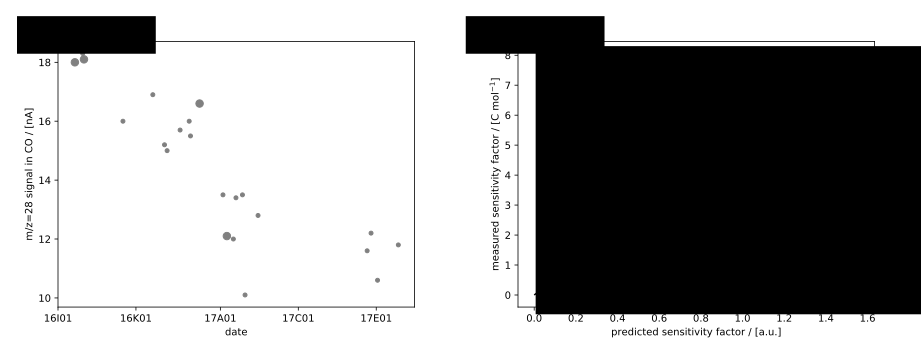
\includegraphics[width=\textwidth]{02_Tools/fig/calibration_results_sniffer2.png}
	\caption{\textbf{(a)}, Signal at m/z=28 with 1 bar \ch{CO} in the membrane chip as carrier gas for experiments done over a period from September 2016 to May 2017. The date on the x-axis is written as \texttt{yyMdd} with \texttt{M}=A representing January, B representing February, etc. \textbf{(b)}, Internal, external, and predicted calibrations for the dataset used in Paper \ref{Trimarco2018}. This is a correction to Figure S6b from the SI of that paper.}
	\label{fig:CuNPs}
\end{figure}

This leads us to the question of \textbf{how often to calibrate}? Figure \ref{fig:CuNPs}a helps answer the question.

This figure includes one data point for each ``successful'' experiment (meaning nothing broke before starting the measurement, results or lack thereof aside - the setup was still under development) during a project that took up most of the first year of my PhD. In that project, which is out of the scope of this Thesis and is, at present, best described in the PhD theses of Anders Bodin\cite{Bodin2017_PhD} and Daniel Trimarco\cite{Trimarco2017_PhD}, we used the EC-MS setup to measure transient phenomena during \ch{CO} reduction on mass-selected, vacuum synthesized copper nanoparticles. Briefly: we drafted an article, included in the appendix to both of those PhD theses, describing how the copper nanoparticles show a transient high selectivity for methane production during the first few seconds of applied potential, whereas ethylene selectivity is more steady. Furthermore, we showed that this methane transient has an independent Tafel slope and depends on prior exposure to air-saturated electrolyte, indicating that oxygen activates the catalytic surface towards a reaction pathway not normally excessible. This was of high interest due to the heated debate in the literature about the effect of oxygen on copper's \ch{CO2} and \ch{CO} reduciton activity\cite{Mistry2016, Gao2017a, Eilert2017, Nitopi2019} (see also, for example, Paper \ref{Scott2019}). We never ended up submitting the draft though, because out of tens of measurements, we were only able to reproduce the result a handful of times (the big dots in Figure \ref{fig:CuNPs}a), with the other experiments showing CO reduction activity not significantly higher than the blank glassy carbon substrate; and we could never see the copper on the sample after the experiment, indicating the nanoparticles were not stable. The work is ongoing, now led by Jakob Ejler, Degenhart Hochfilzer and Ezra Clark. Getting reproducible results on the mass-selected copper nanoparticles is still remarkably challenging, but they are making progress with a patient, systematic approach - in contrast to the brute-force approach that Daniel, Anders, and I had started out with. Figure \ref{fig:CuNPs} was one of my many unsuccessful attempts to find something, ideally within our control, that could separate the ``good results'' from the bad: it shows the m/z=28 signal from the CO carrier gas at the same time during each of those experiments. Unfortunately, it didn't help at all in figuring out what kept going wrong, but it does shed light on the nature of the variability which quantitative mass spectrometry is up against.

Since all of the measurements were made with the same pressure of \ch{CO} flowing through the capillary of chips from the same batch to the same mass spectrometer (which we of course did not tune in the middle of the project), all of the m/z=28 signals should in principle be identical. However, there is both a scatter of +/- approximately 10\% and a gradual drift with a signal loss on the order of 45\% over nine months. The scatter is probably mostly due to the variation in the actual chip capillary dimensions (we were breaking chips quite frequently during that project), but we can't rule out sensitivity effects related to the recent history of the mass spectrometer. The drift is likely due to the mass spectrometer gradually falling out of tune. 

The scatter indicates that it is best to have a calibration on the same day as the measurement. However, calibration of one molecule should be enough, assuming that it is the absolute sensitivity that drifts and not the relative sensitivity. This can be done by internal calibration of one molecule (for example \ch{H2} by HER, which is the inert-gas activity test often used for comparison anyway when studying CO or \ch{CO2} reduciton), or just by measurement of the signal of air or a carrier gas if $l_\text{eff}$ is known for the chip. If an external calibration is used for this purpose, each new chip has to be calibrated - meaning an air measurement through the chip and an OER measurement on the same day (though not necessarily the day of the experiment to be quantified).

The harder work is at the beginning of a project, or if the mass spectrometer is tuned: At that time, make a plot of the type in Figure \ref{fig:CuNPs}b with as many internal and external calibrations as possible. This determines $T(M)$ in case any sensitivity factors need to be predicted in the absence of an internal or external calibration, and gives the relative sensitivities of all the molecules of interest. Then, scale these up or down according to one calibration taken on the day of the measurement. This procedure is facilitated by the \texttt{save\_calibration\_results} and \texttt{save\_calibration\_results} functions of the \ch{EC\_MS} python function. Of course when there is only one analyte of quantitative interest - for example in OER studies - a simple calibration can be done each measurement day and the full calibration results are not strictly necessary. Either way, be aware of how much the sensitivity of the mass spectrometer has drifted - sensitivity factors should not change dramatically from day to day!

To finish up the Section, I will briefly discuss the calibration used for the CO reduciton project mentioned above, which happens to be the same calibration dataset that we published in the SI of Paper \ref{Trimarco2018}:

When studying \ch{CO} reduction, we were most interested in detecting and quantifying methane (\ch{CH4} and ethylene (\ch{C2H4}). \ch{CH4} is best measured at m/z=15 to avoid the interference of \ch{O} at m/z=16, and \ch{C2H4}, at m/z=26 to avoid the shoulder from \ch{CO}. Neither of these products can be made with 100\% Faradaic efficiency by any known electrocatalyst\cite{Hori2008, Qiao2014a}, so internal calibration is not an option. We had \ch{CH4} available as a carrier gas for external calibration, but not \ch{C2H4}. We therefore did internal calibration measurements (\ch{O2}, \ch{H2}, and \ch{CO2}) and external calibration measurements (\ch{O2}, \ch{N2}, and \ch{Ar} in air; \ch{He}, \ch{CO}, and \ch{CH4}), set $l_\text{eff}$ to equate the sensitivity factors measured by internal and external calibration of \ch{O2}, and plotted all of the measured sensitivity factors against the calculated relative sensitivity factors. All of the calibrations fall on approximately the same line, as shown in Figure \ref{fig:CuNPs}b. This enables the prediction of the \ch{C2H4} calibration, indicated by the green dot.

When we published Paper \ref{Trimarco2018}, we had not yet realized that equating the sensitivity factors measured by internal and external calibration of \ch{O2} was the best way to determine $l_\text{eff}$, and instead used a much more convoluted method. With the wrong $l_\text{eff}$, the internal and external calibrations fell on separate lines (Figure S6 of Paper \ref{Trimarco2018}). The procedures described in this Section should therefore be considered an improved and corrected quantification framework when compared to that presented in Paper \ref{Trimarco2018}.


